\begin{document}

O experimento proposto faz uso da interface serial LIN e dos métodos de detecção de erro por bit de paridade, \textit{checksum} e \textit{Cyclic Redudancy Check} (CRC). Essa seção trata cada um desses tópicos em maiores detalhes sobre seu uso e funcionamento.

\subsection{Local Internet Network (LIN)}
\label{fund:lin}

A interface serial \textit{Local Interconnect Network} (LIN), ISO17897, surgiu em 1999 como uma alternativa menos custosa para o \textit{Controller Area Network} (CAN) em redes automotivas \cite{xu2006application}. Isso se deve ao fato de o LIN ter certas características que reduzem o seu custo de implementação. As principais características da rede estão listadas a seguir \cite{popa2006lin, gabriel:2003, xu2006application}:

\begin{itemize}
    \item Um único fio para comunicação;
    \item Comunicação assíncrona, implementada a partir de interfaces comuns -- no caso, \textit{Universal Asynchrounous Receiver/Transmiter} (UART) ou \textit{Serial Communications Interface} (SCI);
    \item Um mestre, múltiplos escravos (\textit{Single Master / Multiple Slave}) -- até 16 escravos;
    \item Até 19,2 Kbits/s;
    \item Máxima distância 40 metros;
    \item Auto-sincronização;
    \item Flexibilidade para adicionar novos \textit{slaves};
    \item Latência garantida entre mensagens;
    \item Possibilidade de \textit{broadcasting} (transmitir o mesmo comando ou mensagem para todos os nós da rede).
\end{itemize}

Com isso, os custos conseguem ser reduzidos pelo uso de apenas um fio e pelo fato de a maioria absoluta dos microcontroladores atuais possuírem alguma interface UART ou SCI \cite{gabriel:2003}.

Em contrapartida, como um único \textit{master} controla toda a rede, caso esse nó esteja comprometido, toda a rede é comprometida \cite{ernst:2018}. Além disso, a taxa de transmissão é muito menor comparada aos 1000 Kbits/s do protocolo CAN.

Sobre os padrões desse protocolo, a comunicação sempre acontece com a mesma estrutura. A Figura \ref{fig:lin_estrutura} extraída de \cite{css:2021} mostra como se dá essa comunicação: sempre o mestre envia um \textit{header} solicitando informação a algum escravo ou enviando algum comando; então, o \textit{slave} correspondente responde com a informação requerida e o \textit{checksum} para proteger contra eventuais falhas na comunicação. Note que apenas o mestre pode iniciar a comunicação no LIN.

\begin{figure*}[htb]
    \centering
    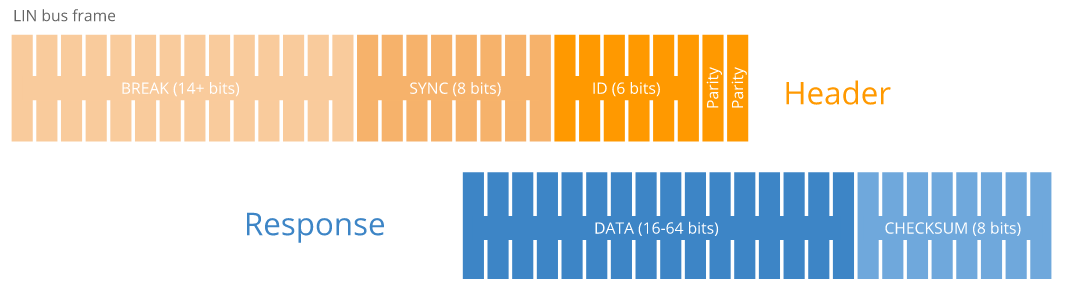
\includegraphics[width=.73\textwidth]{../figs/lin-estrutura}
    \caption{Formato de envio das mensagens em LIN \cite{css:2021}.}
    \label{fig:lin_estrutura}
\end{figure*}

O \textit{header} enviado pelo master é dividido em três partes: primeiro, a linha recebe um \textit{break} que coloca a tensão em nível lógico baixo por um período maior que o requerido para enviar um byte; em seguida é enviado o byte de sincronização (0x55 em hexadecimal, que é uma sequência de 0's e 1's alternados), usado para sincronizar \textit{master} e \textit{slaves}; por último o byte de identificação é enviado. Esse último byte é essencialmente o comando que o mestre está dando para os escravos, sendo que os seis primeiros bits são a informação em si e os dois bits restantes são bits de paridade. O comando pode ser algum especificado pelo próprio protocolo -- como geração de eventos, diagnósticos sobre os \textit{slaves}, comandos definidos pelo usuário ou até códigos reservados -- ou uma solicitação padrão de informação. Nesse caso, é enviado o identificador (ID) do \textit{slave} que deverá enviar as informações que coletou.

Uma vez recebida essa solicitação, o escravo verifica se ele deverá responder ou ignorar a mensagem recebida. No caso de o ID coincidir com o seu, este envia as informações que possui. Esse dado pode ter de dois a oito bytes, sendo que essa quantidade é predefinida de acordo com o ID do \textit{slave} (certas faixas enviam dois bytes, outras três, e assim por diante). Por fim, é enviado o \textit{checksum} para que o mestre possa identificar eventuais erros na mensagem recebida.

Já sobre os aspectos elétricos do protocolo, a tensão de operação na linha é de 12V. Para o emissor, uma margem de 20\% nos níveis de tensão é estabelecida, sendo que para o receptor essa margem é de 40\% \cite{ti2018lin}. Um nível lógico alto representa uma tensão próxima de 12V, enquanto que um nível lógico baixo representa valores próximos de 0V.

A Figura \ref{fig:linconect} obtida em \cite{ti2018lin} mostra como ocorre a conexão entre mestre e escravos no LIN. Pode-se perceber que, nessa situação, o transceptor LIN é comandado pelo microcontrolador por meio de SCI, enquanto que os transceptores LIN trocam informações entre si por um único fio.

\begin{figure}[htb]
    \centering
    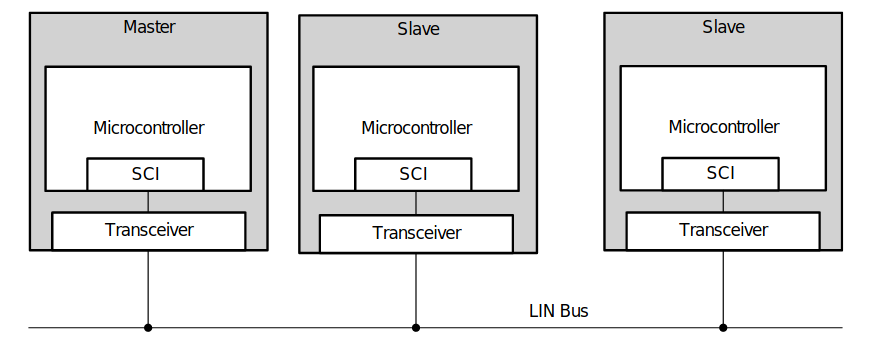
\includegraphics[width=.5\textwidth]{../figs/linconect}
    \caption{Estrutura de uma rede LIN \cite{ti2018lin}.}
    \label{fig:linconect}
\end{figure}

Portanto, o LIN especifica várias camadas do protocolo, que vão desde a camada física até a aplicação. Com esse padrão bem definido, componentes de qualquer fabricante devem operar corretamente em conjunto e critérios de interoperabilidade podem ser alcançados.

\subsection{Métodos de Detecção de Erro}
\label{fund:erros}

Naturalmente, durante a comunicação entre dispositivos podem ocorrer interferências na linha e erros na mensagem acabam surgindo. A fim de identificar esses erros, existem os métodos de detecção que adicionam informações extras à mensagem, trazendo maior confiabilidade para a rede.

Dois métodos foram utilizados nesse projeto: o \textit{checksum} e o \textit{Cyclic Redundancy Check} (CRC). Cada um deles será apresentado em maiores detalhes a seguir.

\subsubsection{Bit de Paridade}

Um dos métodos mais simples de detecção de erros é o bit de paridade. A ideia é adicionar bits a uma mensagem de modo que a soma de todos os bits seja um valor par ou ímpar \cite{rahmani2007error}. Assim, apenas um número ímpar de erros pode ser identificado corretamente.

Existe, portanto, uma separação entre paridade ímpar e paridade par, sendo cada variante do método previamente definida pelo protocolo ou sistema. No caso do LIN, utiliza-se a paridade par \cite{ti2018lin} construída sobre os dois bits finais do byte identificador -- como é possível perceber na Figura \ref{fig:lin_estrutura}.

Dadas essas características do método, esse é utilizado em situações nas quais o tempo de processamento é restrito, mas existe uma margem maior para erros na troca de dados.

\subsubsection{\textit{Checksum}}
Já o \textit{checksum} traz uma sensibilidade melhorada para a detecção de erros em comparação ao bit de paridade \cite{rahmani2007error}. Para esse método, os valores são somados byte a byte, e o resultado da soma é invertido (cada bit zero se adquire o valor um e vice-versa) e então enviado. Vale ressaltar que o tamanho para esse valor enviado é fixo, sendo que comumente são adotados \textit{checksum}s de 8, 16 e 32 bits.

No decodificador, a soma é feita tanto para os bytes da mensagem quanto para o \textit{checksum} recebido. Após a inversão do resultado, espera-se que o valor obtido seja nulo, de modo que nenhum erro tenha sido identificado na mensagem. Caso contrário, houve um erro na comunicação.

Para o protocolo em questão, o \textit{checksum} é adotado como parte de sua estrutura, sendo enviado em toda resposta do escravo. Um byte é o tamanho da informação adicional, portanto têm-se um \textit{checksum} de 8 bits no LIN.

\subsubsection{Cyclic Redundancy Check (CRC)}

O \textit{Cyclic Redudancy Check} (CRC) é um algoritmo baseado na divisão polinomial em base 2 \cite{errors1995crcchecksum}. Por meio de operações XOR (ou exclusivo) acontece a divisão da mensagem a ser enviada (\textit{dataword}) pelo polinômio gerador. O resto dessa divisão é adicionado à mensagem, formando a \textit{codeword}. Na decodificação, a \textit{codeword} é dividida pelo polinômio gerador e, caso o resto (síndrome) for nulo, a mensagem foi enviada corretamente.

Existem diversos algoritmos para o CRC, variando o tamanho da mensagem a ser avaliado e o gerador. No caso em questão, como apenas um byte de informação compõe a \textit{dataword}, o CRC-8 foi utilizado (oito bits ou um byte). Já o polinômio gerador foi o valor 0xD5 em hexadecimal, e esse valor tabelado cumpre os requisitos para que o CRC possa identificar erros de bit corretamente.

Também é possível implementar o CRC com uma abordagem baseada em uma tabela. Como a lista de valores possíveis de \textit{dataword} para o CRC não é muito extensa, pode-se consultar qual o valor a ser adicionado à mensagem em uma tabela contendo essas relações. Ao final, o resultado obtido é o mesmo, porém com melhor desempenho em questão de tempo de execução, ao custo de um maior uso de memória.

\end{document}